\documentclass{beamer}

%\setbeamertemplate{note page}[plain]
%\setbeameroption{show notes} 

\usepackage{physics}

\usepackage{amsmath}
\usepackage{tikz}
\usetikzlibrary{tikzmark}
\setbeamertemplate{caption}[numbered]

\newcommand{\nl}{\\ \vspace{1em}}

\mode<presentation> {

% The Beamer class comes with a number of default slide themes
% which change the colors and layouts of slides. Below this is a list
% of all the themes, uncomment each in turn to see what they look like.

%\usetheme{default}
%\usetheme{AnnArbor}
%\usetheme{Antibes}
%\usetheme{Bergen}
%\usetheme{Berkeley}
%\usetheme{Berlin}
%\usetheme{Boadilla}
%\usetheme{CambridgeUS}
%\usetheme{Copenhagen}
%\usetheme{Darmstadt}
%\usetheme{Dresden}
%\usetheme{Frankfurt}
%\usetheme{Goettingen}
%\usetheme{Hannover}
\usetheme{Ilmenau}
%\usetheme{JuanLesPins}
%\usetheme{Luebeck}
%\usetheme{Madrid}
%\usetheme{Malmoe}
%\usetheme{Marburg}
%\usetheme{Montpellier}
%\usetheme{PaloAlto}
%\usetheme{Pittsburgh}
%\usetheme{Rochester}
%\usetheme{Singapore}
%\usetheme{Szeged}
%\usetheme{Warsaw}

% As well as themes, the Beamer class has a number of color themes
% for any slide theme. Uncomment each of these in turn to see how it
% changes the colors of your current slide theme.

%\usecolortheme{albatross}
%\usecolortheme{beaver}
%\usecolortheme{beetle}
%\usecolortheme{crane}
%\usecolortheme{dolphin}
%\usecolortheme{dove}
%\usecolortheme{fly}
%\usecolortheme{lily}
%\usecolortheme{orchid}
%\usecolortheme{rose}
%\usecolortheme{seagull}
%\usecolortheme{seahorse}
%\usecolortheme{whale}
%\usecolortheme{wolverine}

%\setbeamertemplate{footline} % To remove the footer line in all slides uncomment this line
%\setbeamertemplate{footline}[page number] % To replace the footer line in all slides with a simple slide count uncomment this line

%\setbeamertemplate{navigation symbols}{} % To remove the navigation symbols from the bottom of all slides uncomment this line
}

\usepackage{graphicx} % Allows including images
\usepackage{booktabs} % Allows the use of \toprule, \midrule and \bottomrule in tables

%----------------------------------------------------------------------------------------
%	TITLE PAGE
%----------------------------------------------------------------------------------------

\title[Quantum Love]{Quantum Love: \\ The Interplay of Science with Emotion} % The short title appears at the bottom of every slide, the full title is only on the title page

\author{Daniel Prelipcean} % Your name
\institute[JUB Stem Slam 2018] % Your institution as it will appear on the bottom of every slide, may be shorthand to save space
{Jacobs University Bremen
 \\ % Your institution for the title page
\medskip
\textit{d.prelipcean@jacobs-university.de} % Your email address
}
\date{\today} % Date, can be changed to a custom date

\begin{document}

\begin{frame}
\titlepage % Print the title page as the first slide

\note{Physics is like sex}

\end{frame}



%----------------------------------------------------------------------------------------
%	PRESENTATION SLIDES
%----------------------------------------------------------------------------------------

%------------------------------------------------
\section{Introduction} % Sections can be created in order to organize your presentation into discrete blocks, all sections and subsections are automatically printed in the table of contents as an overview of the talk


%----------------------------------------------------------------------------------------



\begin{frame}


\frametitle{Physics is Fun!}
\begin{columns}
\column{0.5\textwidth}
"Physics is like sex: sure, it may give some practical results, but that's not why we do it."
\nl
\uncover<2->{(Richard Feynman)}

\column{0.5\textwidth}
\begin{figure}
\uncover<2->{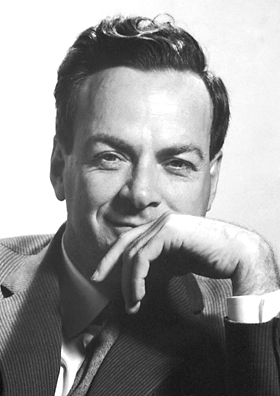
\includegraphics[scale=0.35]{Pics/Richard_Feynman_Nobel.jpg}
\caption{Nobel Prize Picture \footnotemark}}
\end{figure}
\end{columns}

\only<2->{\footnotetext[1]{wikipedia}}


    
\end{frame}

%------------------------------------------------

\begin{frame}


\frametitle{Motivation and Idea}


\begin{figure}
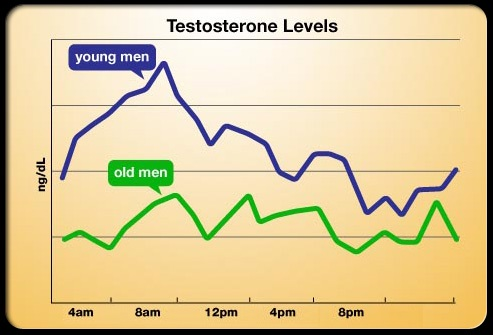
\includegraphics[width=0.5\textwidth]{Pics/Low-Testosterone-Symptoms.jpg} 
\caption{Male Testosterone Levels \footnotemark}
\label{pic:maletestosteroneleveles}
\end{figure}

\only<2->{\footnotetext[2]{become-the-alpha-male.com/blog/category/testosterone/}}




\note{Here is an interesting graph about male`s testosterone levels as functions of time throughout the day. The male organism has a hormonal peak in the morning and then it widely fluctuates. That is why gentlem enare especially horny when they wake up.

Coincidentally, the quantum physics lectures at Jacobs are also in the morning, and so you end up with a classroom full of horny physicists, learning about how to get excited states. 
In of these lecture, the idea of Quantum Sex appeared, and hence this presentation.}

\end{frame}

%------------------------------------------------

\begin{frame}
\frametitle{Disclaimer}

\uncover<2->{
If you feel offended, let me know such that I can skip the respective part of my presentation.

\nl
If you feel offended, but do not want to speak up, let me know afterwards, such that I can change it and improve in future presentations.
}

    
\end{frame}


%------------------------------------------------

\section{Wavefunctions} % A subsection can be created just before a set of slides with a common theme to further break down your presentation into chunks

\begin{frame}

\frametitle{Basics of Quantum Mechanics}
The main object in Quantum Mechanics is the wavefunction $\psi$.

\uncover<2->{
Employing Dirac notation, this is written as:
}
\begingroup
\huge
\begin{align*}
\onslide<4->{\tikzmark{a}\hat{\mathbb{O}}}\uncover<2->{ \ket{\psi}} & \onslide<5->{=\tikzmark{b} o  \ket{\psi}}
\end{align*}

\begin{equation*}
\onslide<8->{\widehat{Feeling}} \onslide<7->{\vcenter{\hbox{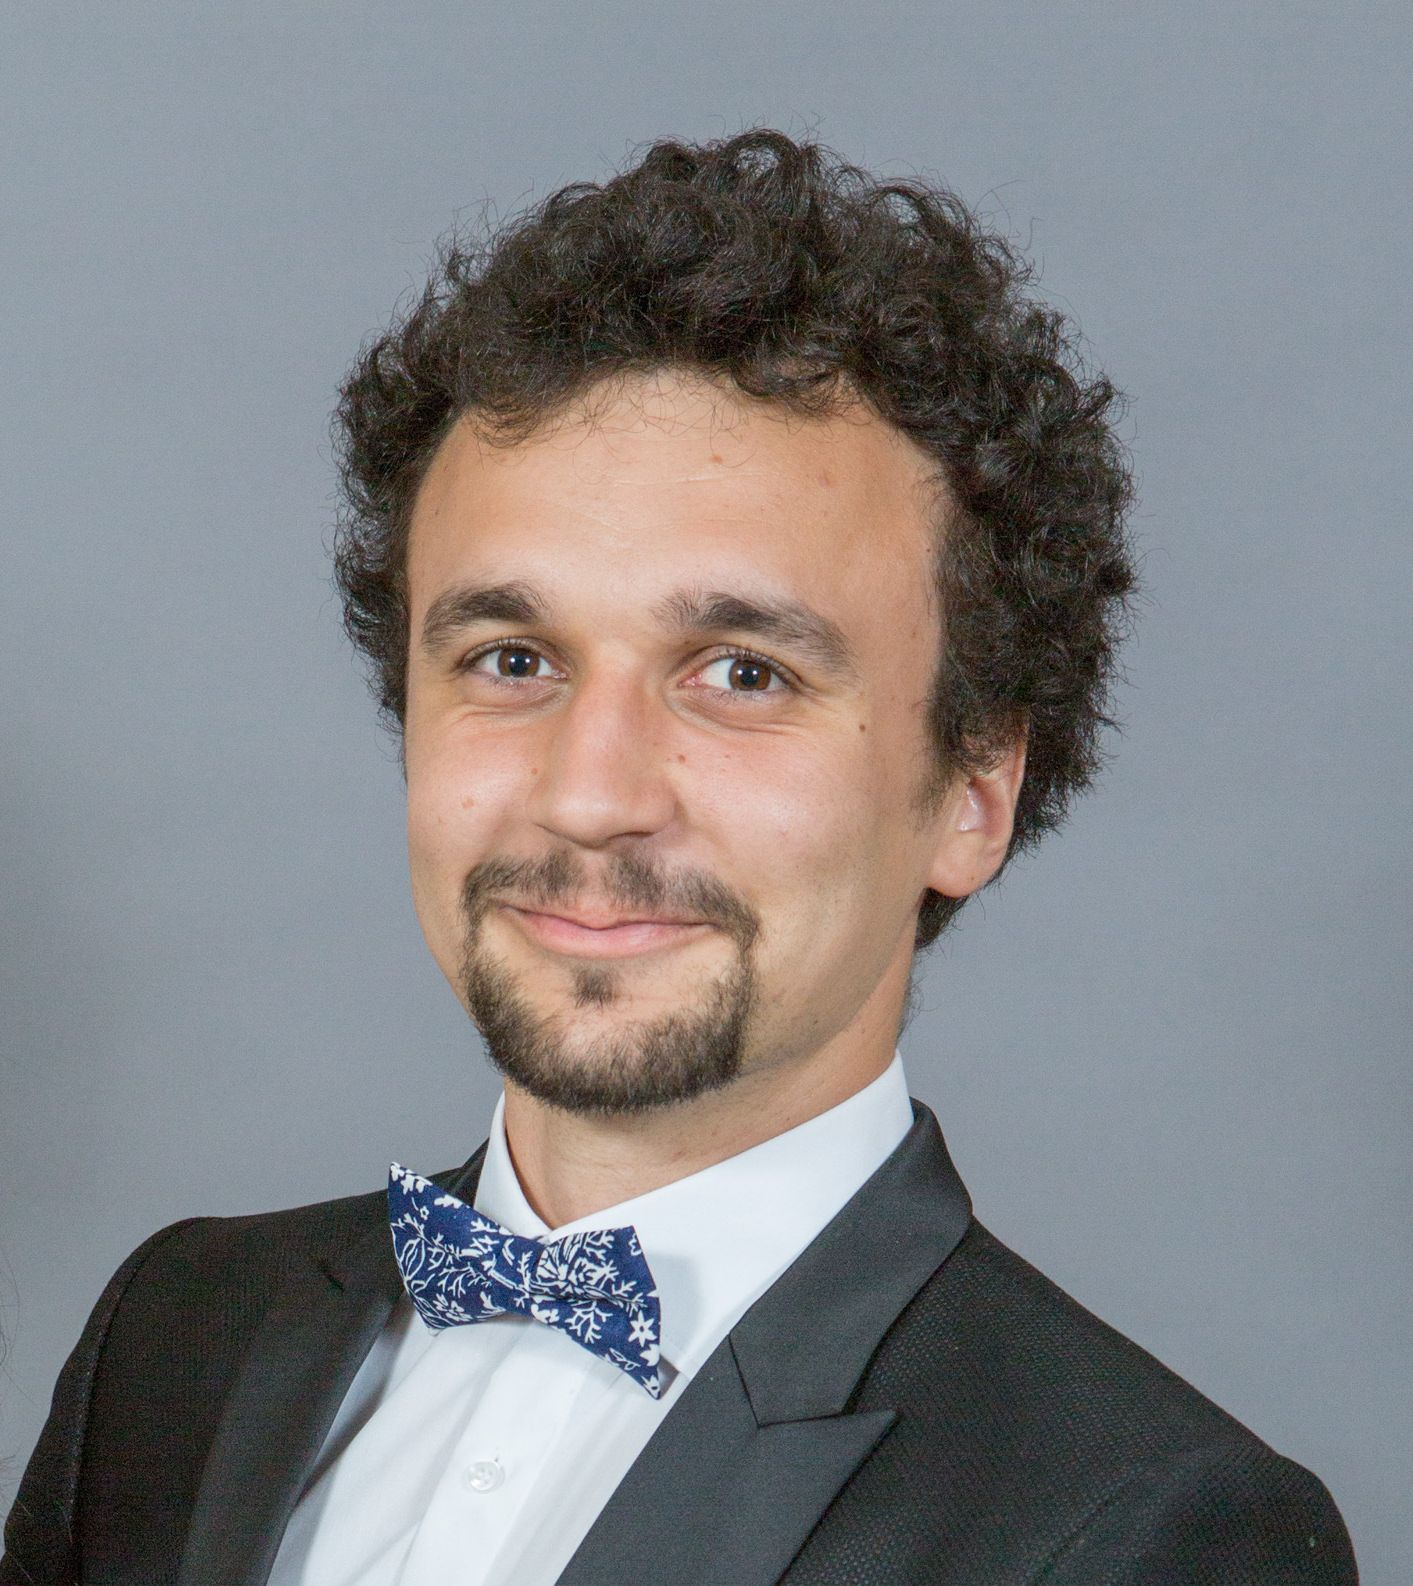
\includegraphics[width=0.2\textwidth]{Pics/pic_me.jpg}}}} \onslide<9->{=\text{nervous} \vcenter{\hbox{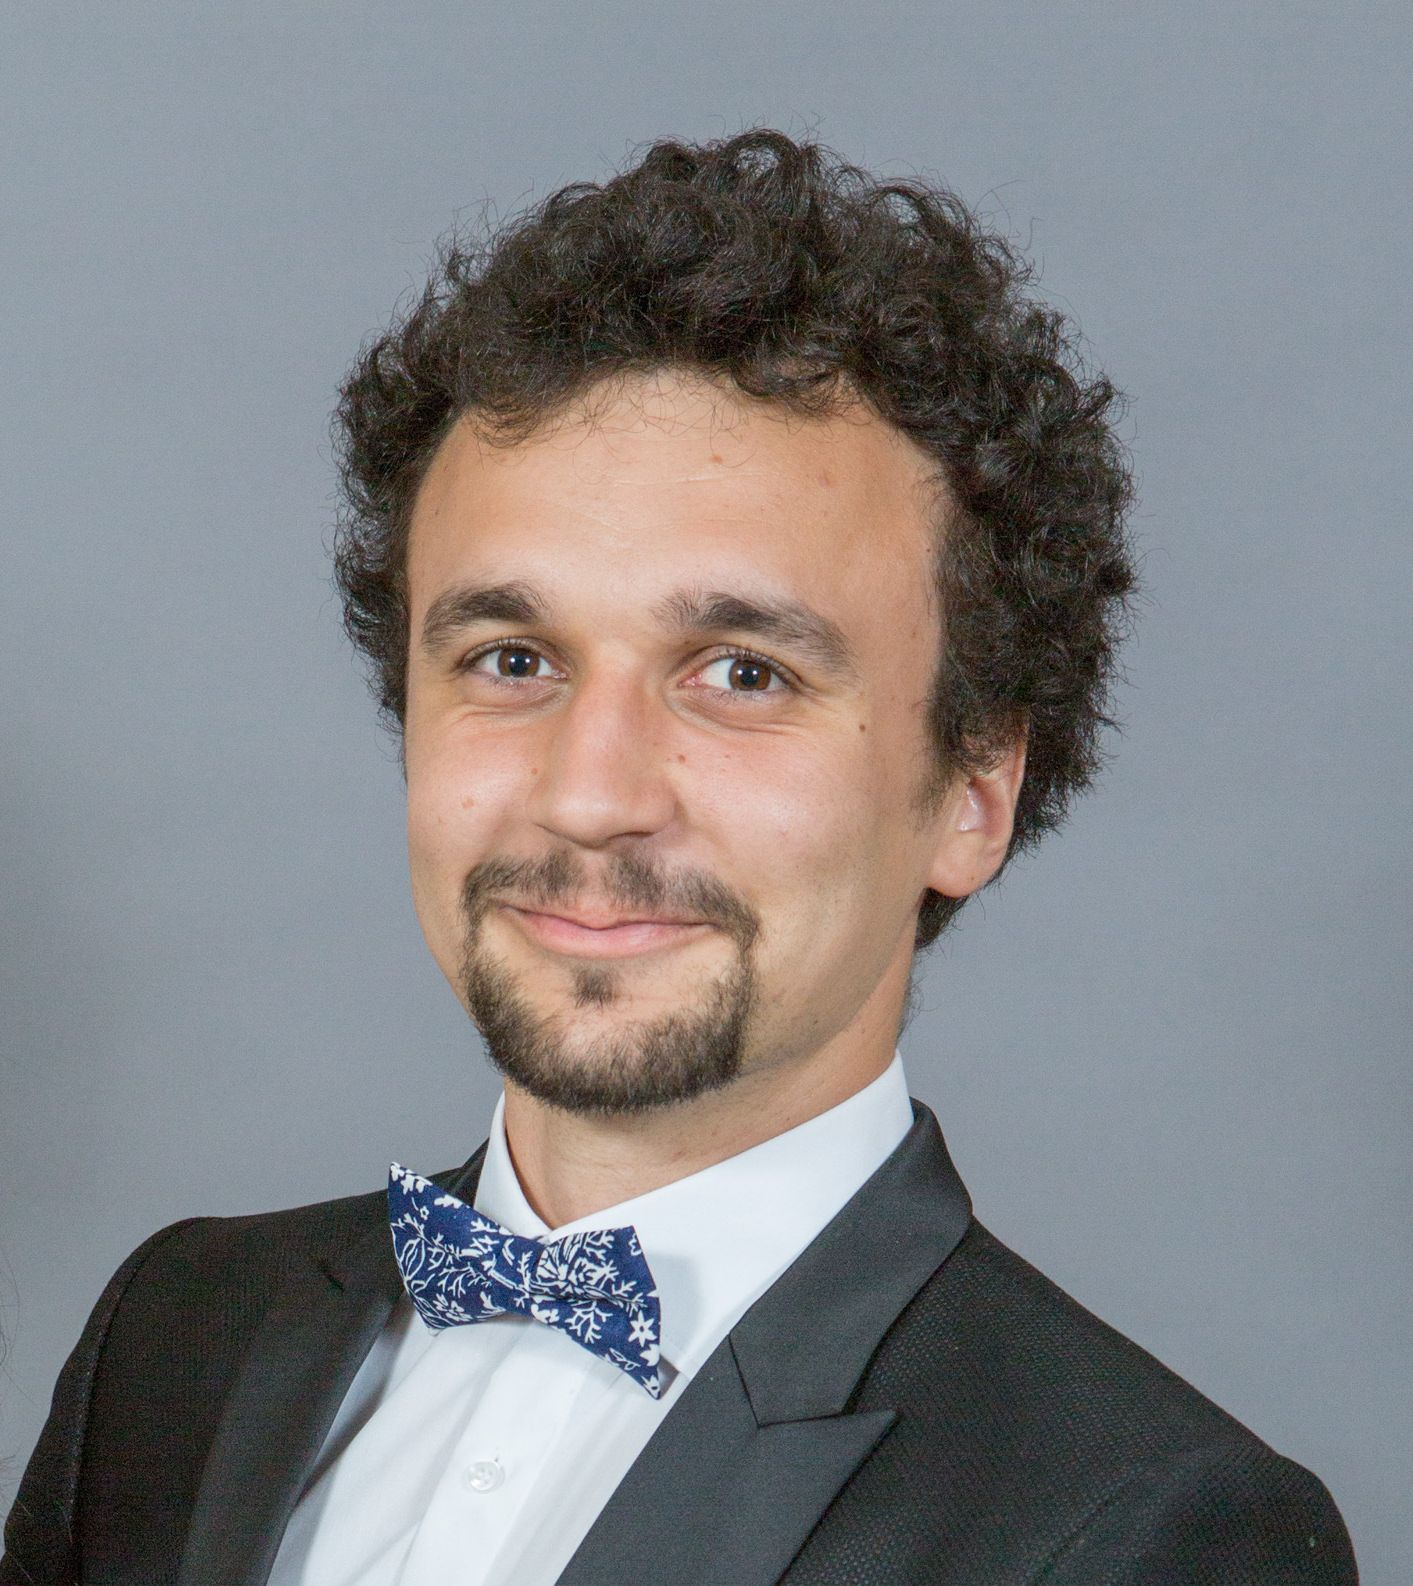
\includegraphics[width=0.2\textwidth]{Pics/pic_me.jpg}}}}
\end{equation*}

\uncover<6->{
\begin{tikzpicture}[remember picture,overlay]
\draw[<-] 
   ([shift={(10pt,-5pt)}]pic cs:a) |- ([shift={(-10pt,-15pt)}]pic cs:a) 
  node[anchor=east] {$\scriptstyle \text{operator}$};  
\draw[->] 
  ([shift={(10pt,-5pt)}]pic cs:b) |- ([shift={(20pt,-15pt)}]pic cs:b) 
  node[anchor=west] {$\scriptstyle \text{eigenvalue}$}; 
 
\end{tikzpicture}
}
\endgroup



\note{Fourier transform: position-momentum space with gentlemen-ladies space}

    
\end{frame}

%----------------------------------------------------------------------------------------

\begin{frame}
\frametitle{States Spaces}
Superposition Principle: Male State Space
\begin{equation}
\ket{m(x)}= \sum_{i=0}^n c_i \ket{m_i(x)}
\end{equation}

%\begingroup
%\huge
%\begin{equation*}
%\uncover<2->{\vcenter{\hbox{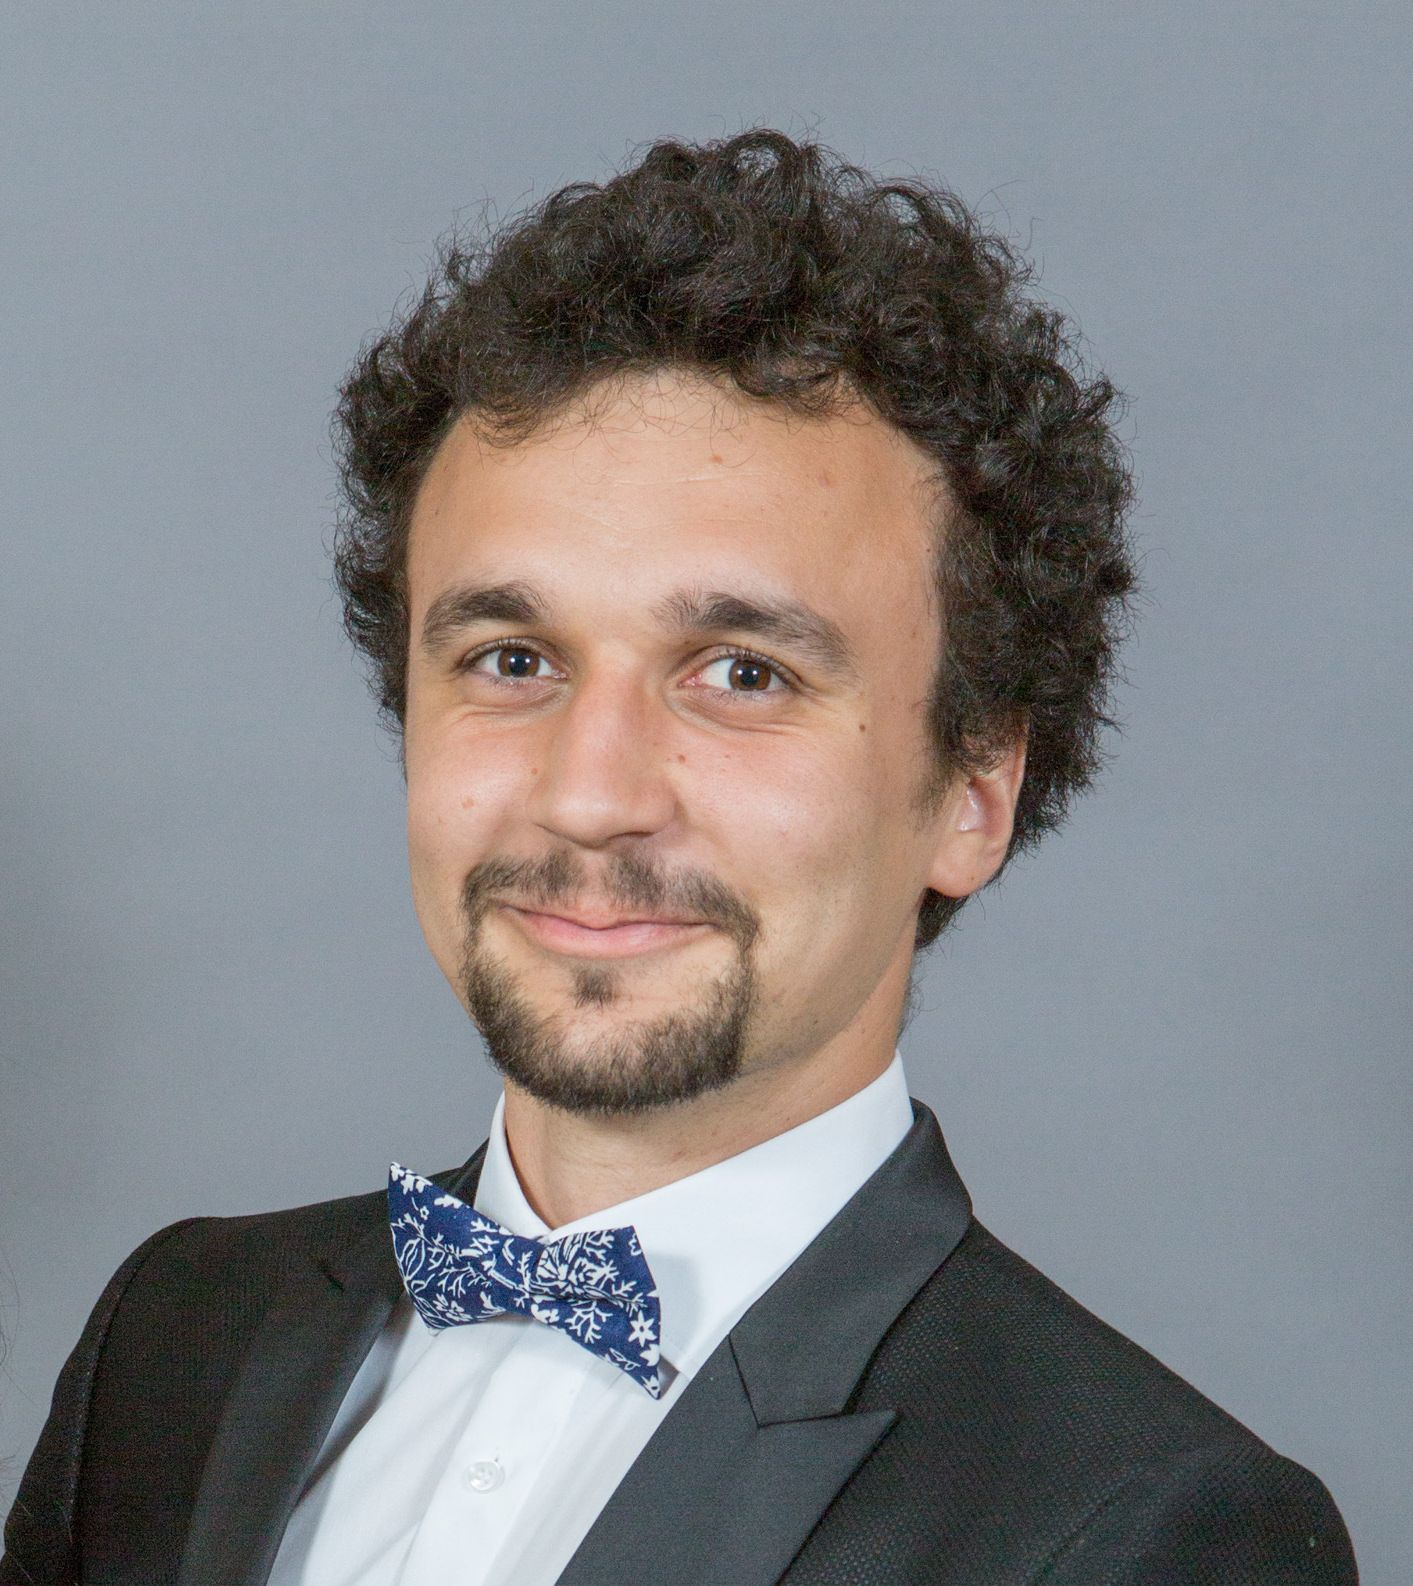
\includegraphics[width=0.15\textwidth]{Pics/pic_me.jpg}}}} \uncover<3->{= c_1 \vcenter{\hbox{\includegraphics[width=0.15\textwidth]{Pics/face.jpg}}}} \uncover<4->{ + c_2 \vcenter{\hbox{\includegraphics[width=0.15\textwidth]{Pics/crop.JPG}}}} \uncover<5->{ + c_3 \vcenter{\hbox{\includegraphics[width=0.15\textwidth]{Pics/profile_pic_Face.png}}}} \uncover<6->{ + \hdots}
%\end{equation*}
%\endgroup

\end{frame}



%----------------------------------------------------------------------------------------

\begin{frame}
\frametitle{Fourier transform between gentlemen and ladies space}

\begin{equation}
\uncover<2->{\ket{w(k)} =} \uncover<1->{\sum_j c_j} \uncover<4->{ \frac{1}{(\sqrt{2\pi})^d} \int  d^d x} \ \uncover<1->{\ket{m_j(x)}} \uncover<3->{e ^{-i k x}} \uncover<5->{\delta(k_\mu k^\mu + m^2)} \uncover<6->{ \Theta(k_\mu x^\mu) }
\end{equation}

\uncover<2->{
where:}
\begin{enumerate}
\uncover<3->{\item the exponential = our first attempt to understand something }

\uncover<4->{\item $d$ dimensions = cannot even comprehend in how many ways a woman can think }

\uncover<5->{\item the delta function $\delta$ = engage in a conversation only when appropriate }

\uncover<6->{\item step function $\Theta(\mu)$ = apologize when mistaken }


\end{enumerate}

\note{Being male, it is very convenient for me to work in the male space.

But the female space is a complete unknown for me:

And this bring a lot of complications along the way}

    
\end{frame}

%----------------------------------------------------------------------------------------
\section{Operators}

\begin{frame}
\frametitle{The Love operator}

\uncover<2->{Let $\hat{L}$ be the Love operator, with the desired property:}

\uncover<3->{
\begin{equation}
\hat{L} \ket{w} = \text{(loves me)} \ket{w}
\end{equation}
}

\uncover<4->{Problem: Hard to find exact representation of $\hat{L}$ for different ladies $\ket{w_j}$.}
\nl
\uncover<5->{\textbf{Daniel`s Conjecture:}} \uncover<6->{One can find a suitable representation of $\hat{L}$ only for a single woman $\ket{w} = \ket{g}$, that is, the girlfriend.}

\end{frame}
%----------------------------------------------------------------------------------------


\begin{frame}
\frametitle{Common Approximations (1)}
\begin{equation*}
\uncover<2->{\hat{L} \ket{w}}\uncover<3->{ \approx \widehat{\text{Flowers}} \ket{w} } \uncover<4->{ = \text{impressed} \ket{w}}
\end{equation*}

\begingroup
\Large
\begin{equation*}
\uncover<6->{\widehat{\text{Flowers}}} \uncover<5->{\vcenter{\hbox{\includegraphics[width=0.15\textwidth]{Pics/Nicoleta.jpg}}}} \uncover<7->{=  \vcenter{\hbox{\includegraphics[width=0.15\textwidth]{Pics/flowers.JPG}}}}  \uncover<8->{= \vcenter{\hbox{\includegraphics[width=0.15\textwidth]{Pics/impre.JPG}}}} 
\end{equation*}
\endgroup

\end{frame}
%----------------------------------------------------------------------------------------


\begin{frame}
\frametitle{Common Approximations (2)}
\begin{equation*}
\uncover<2->{\hat{L} \ket{w}}\uncover<3->{ \approx \widehat{\text{Romantic Dinner}} \ket{w} } \uncover<4->{ = \text{impressed} \ket{w}}
\end{equation*}

\begingroup
\Large
\begin{equation*}
\uncover<6->{\widehat{\text{Romantic Dinner}}} \uncover<5->{\vcenter{\hbox{\includegraphics[width=0.15\textwidth]{Pics/Nicoleta.jpg}}}} \uncover<7->{=  \vcenter{\hbox{\includegraphics[width=0.15\textwidth]{Pics/dinner.jpg}}}}  \uncover<8->{= \vcenter{\hbox{\includegraphics[width=0.15\textwidth]{Pics/impre.JPG}}}} 
\end{equation*}
\endgroup


\note{What I was particularly interested in is the love operator.
Usually, one knows how to apply it to oneself, but no to other people. Meaning that it is hard to find the exact representation of this operator for different partners.}



    
\end{frame}
%----------------------------------------------------------------------------------------

\begin{frame}
\frametitle{The Cheating operator}
\uncover<2->{
Operators may change the state completely, e.g. the cheating operator $\hat{C}$. 
}
\nl
\uncover<3->{
Let $\ket{g}$ be your girlfriend, and $\ket{w}$ be another girl. Then:
\begin{equation}
    \hat{S} \ket{w} = \hat{C} \ket{g} = \uncover<4->{0 \ket{0} = 0}
\end{equation}
}

\uncover<4->{For eternity.}
\nl
\uncover<5->{\textbf{Conclusion:} Not all operator equations are eingenvalue problems.}
\note{If you have sex with another girl, which qualifies as cheating and if your girlfriend finds out, which she always does, then you lose your girlfriend. So the state collapses to 0.

Moreover, you are not the only one acting on these states, so they may change without notice. That is why, one has to act rather quickly
}
    
\end{frame}
%----------------------------------------------------------------------------------------


\begin{frame}
\frametitle{The Sex operator }
\uncover<2->{
Let $\hat{S}$ be the sex operator, with the desired property:
\begin{equation}
\hat{S} \ket{g} = \text{sex} \ket{g}
\end{equation}
}

\uncover<3->{
However, it can be the case that:
\begin{equation}
    \hat{S} \ket{g} =\text{harrasment} \ket{g}
\end{equation}
So be very careful with this one!
}
\nl
\uncover<4->{\textbf{Hopeful Lemma:} As $t \to \infty$, the above case will happen with probability $P= 0$, that is, never again.}

\end{frame}
%----------------------------------------------------------------------------------------


\begin{frame}
\frametitle{The Sex operator }

Practically, one may have to apply it multiple times to reach the desired result:
\begin{equation}
\hat{S}^n \ket{g} = \text{sex} \ket{g}
\end{equation}

\uncover<2->{Scientists are especially interested in limit cases:}

\uncover<3->{
e.g. $n = 0$, i.e. you do not have to do anything and get:

\begin{equation}
\hat{S}^0 \ket{g} = \ket{g} = sex \ket{g}
\end{equation}
}

\uncover<4->{\textbf{Open question:} Prove whether such states exist (or not).}

\note{As a side note, there are people who are more physical, so they are interested in the sex operator $\hat{S}$, but it may happen that this operator cannot be always applied! So be very careful with this one.
As physicists, we are interested in the limiting cases to find inconsistencies or evidence. 
I still have to prove that such girls exist.
}    
    
\end{frame}
%----------------------------------------------------------------------------------------



\begin{frame}
\frametitle{The Love operator (yet again) }
\uncover<2->{A more realistic scenario is the following:

\begin{equation}
    \hat{L}^n \ket{g} =  \Pi_{j=1}^N (L_j)  \ket{g} = \text{(in love)} \ket{g}
\end{equation}
}

\uncover<3->{That is, one has to apply it multiple times, possibly using different representations or common approximations (as before).}
\nl
\uncover<4->{
Most interesting case: $n \to \infty$.}
\nl
\uncover<5->{
\textbf{Problem:}\\ How to apply an infinite amount of work?} \uncover<6->{($\approx 0 $ in her eyes)}

\end{frame}
%----------------------------------------------------------------------------------------



\begin{frame}
\frametitle{The Love operator solution}

\uncover<2->{
Answer: Apply the Interest operator $\hat{I}$:
\begin{equation}
    \hat{I} \ket{g} = \text{(interested in me)}\ket{g}
\end{equation}
}

\uncover<3->{
such that she wants to apply to Love operator on me, that is:
\begin{equation}
    \item \hat{L}_{w} \ket{b} = \text{(?)} \ket{b}
\end{equation}
}

    

\end{frame}

%----------------------------------------------------------------------------------------



\begin{frame}
\frametitle{Conclusion}
Quantum Physics in a nutshell:
\begin{enumerate}
    \pause \item Define your wave functions in a suitable basis.
    \pause \item Investigate how operators apply on the wave functions (and pay much attention how you can apply them).
    \pause \item Obtain physical results that can be experimentally achieved.
\end{enumerate}




    
\end{frame}

%----------------------------------------------------------------------------------------



\section{Conclusion}

\begin{frame}
\frametitle{Acknowledgements}

\begin{columns}
\column{0.5\textwidth}
\uncover<2->{
\begin{figure}
\includegraphics[scale=0.10]{Pics/grad.JPG}
\caption{Success! $(n \gg 1)$}
\end{figure}}
\column{0.65\textwidth}

I acknowledge \uncover<2->{psychological support from my girlfriend  Nicoleta (JUB, Class of 2017)} \uncover<3->{and financial support from my parents, through the Grant RO-B961217.

\begin{figure}
\includegraphics[scale=0.065]{Pics/fam.jpg}
\caption{Prelipcean Family}
\end{figure}}
\end{columns}





\note{For those who knew QM from before, I hope you enjoyed this. For those who did not know, I hope that you know have an idea what QM is all about.

To end, I would like to share with all of you the following message:

Science is the most beautiful endeavour mankind has ever done.

Thank you!
}    
    
\end{frame}

%----------------------------------------------------------------------------------------

\begin{frame}
\frametitle{Take Home Message}

\uncover<2->{Humans} \uncover<3->{= social beings, who urge to feel love. }

\nl

\uncover<4->{Tell "I love you" more often, and louder!}



\nl

\uncover<5->{Even the most aesthetic equation cannot compare to a sincere \\
"I love you" \\
from your loved ones.}

\nl

\uncover<6->{Thank You and May the Force be with You!}

    
    
\end{frame}
%----------------------------------------------------------------------------------------


\end{document}